% !TeX encoding = UTF-8
% !TeX program  = pdflatex

\documentclass[xcolor={svgnames,table},10pt,fleqn]{beamer}
\usepackage{stb-beamer-a}

%---- AMS math ---------------------------------------------------------
\usepackage{amsmath,amsthm}

%---- Fonts ------------------------------------------------------------
\usefonttheme{professionalfonts}

\usepackage[T1]{fontenc}
\usepackage{textcomp}
\usepackage[default,medium,scaled=1.0]{raleway}
\usepackage[scaled=0.80]{arevmath}

%---- Packages ---------------------------------------------------------

\usepackage{tikz}
\usepackage{booktabs}
\cmidrulewidth=\heavyrulewidth

\graphicspath{{figs/}}

%---- Title page -------------------------------------------------------

\title[\footnotesize Ballistic\\ Gel]
      {\Large DEM Modeling of Ballistic Gelatin for Low Energy Impacts}
%\subtitle{}

\author{{\bfseries HC Grobbelaar\and DNJ Els\and CJ Coetzee}}
\institute{\itshape Dept of Mech \& Mechatronic Eng,\\
           Stellenbosch University, South Africa}

\date{4th Aspherix and CFDEM Conference\\[0.5ex]
      \small 20--21 Apr 2023, Linz, Austria}

\def\titlefig{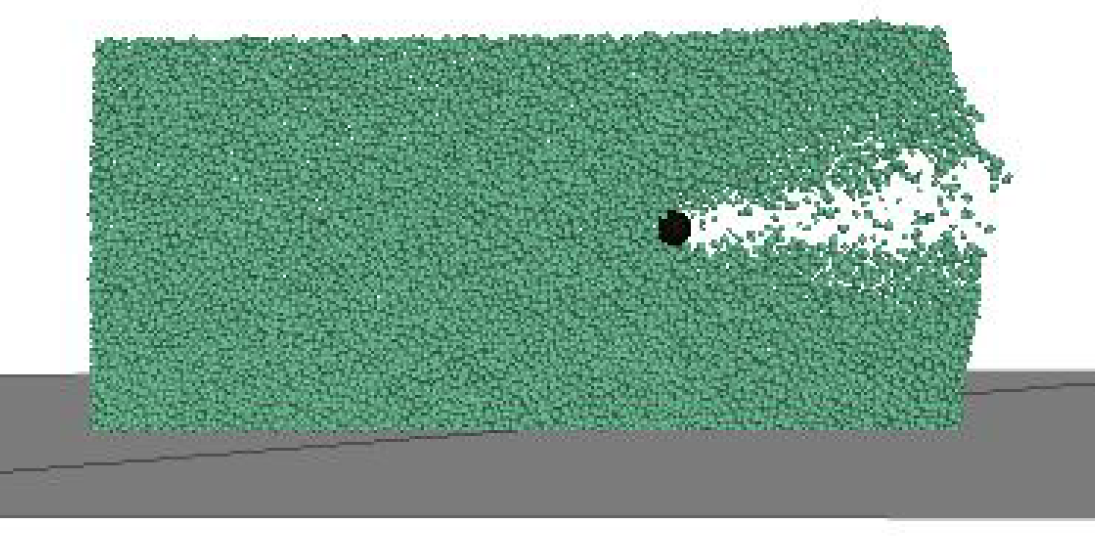
\includegraphics[width=7.0cm]{Ball-penetrate}}

%====================================================================
\begin{document}
\begin{frame}
  \maketitle
\end{frame}

%\begin{frame}
%    \begin{alertblock}{COPYRIGHT}
%    Copyright \textcopyright\ 2023 Stellenbosch University\\
%    All rights reserved
%    \end{alertblock}
%\end{frame}


\begin{frame}
  \frametitle{Contents}
  \tableofcontents
\end{frame}

%=====================================================================
\section{Blocks}

\begin{frame}{Blocks}
\begin{block}{General block}
    A general block ...
\end{block}
\begin{alertblock}{Alert block}
    An alert block ...
\end{alertblock}
\begin{exampleblock}{Example block}
    An example ...
\end{exampleblock}
\begin{theorem}[Theorem block]
    A theorem ...
\end{theorem}
\end{frame}

%=====================================================================
\section{Colours}

\begin{frame}{STB Colours}
\begin{center}
\begin{tabular}{llr@{}r@{ }r@{ }r@{}r@{}}
 & \textbf{Color name} & \multicolumn{5}{c}{\textbf{RGB}} \\[0.25ex]
 \cmidrule(lr){2-2}
 \cmidrule(l){3-7}
\colorbox{stbMaroon}{\phantom{XXXXX}} & {stbMaroon} &(&  97,&  34,&  59&) \\[0.25ex]
\colorbox{stbGold}  {\phantom{XXXXX}} & {stbGold}   &(& 183,& 153,&  98&) \\[0.25ex]
\colorbox{stbGreen} {\phantom{XXXXX}} & {stbGreen}  &(& 130,& 204,& 174&) \\[0.25ex]
\colorbox{stbOrange}{\phantom{XXXXX}} & {stbOrange} &(& 220,&  68,&   5&) \\[0.25ex]
\colorbox{stbWine}  {\phantom{XXXXX}} & {stbWine}   &(& 166,&  10,&  61&) \\[0.25ex]
\colorbox{stbSoil}  {\phantom{XXXXX}} & {stbSoil}   &(& 100,&  51,&  53&) \\
\end{tabular}
\end{center}
\end{frame}


%=====================================================================
\section{Lists}
\begin{frame}{Lists}
\begin{block}{Itemize}
\begin{itemize}
    \item First item
    \item Second item
    \item ...
\end{itemize}
\end{block}
\begin{block}{Enumerate}
\begin{enumerate}
    \item First item
    \item Second item
    \item ...
\end{enumerate}
\end{block}
\begin{block}{Description}
\begin{description}
    \item[First item] ...
    \item[Second item] ...
    \item [...] ...
\end{description}
\end{block}

\end{frame}



%=====================================================================
\section{Math}

\begin{frame}{Math}
\begin{block}{Residue Theorem}
Let $f$ be analytic in the region $G$ except for the isolated singularities $a_1,a_2,\ldots,a_m$. If $\gamma$ is a closed rectifiable curve in $G$ which does not pass through any of the points $a_k$ and if $\gamma\approx 0$ in $G$ then
\[
\frac{1}{2\pi i}\int_\gamma f = \sum_{k=1}^m n(\gamma;a_k) \text{Res}(f;a_k).
\]
\end{block}

Another nice theorem from complex analysis is

\begin{block}{Maximum Modulus}
Let $G$ be a bounded open set in $\mathbb{C}$ and suppose that $f$ is a continuous function on $G^-$ which is analytic in $G$. Then
\[
\max\{|f(z)|:z\in G^-\}=\max \{|f(z)|:z\in \partial G \}.
\]
\end{block}
\end{frame}



%=====================================================================

\begin{frame}[plain]
\begin{tikzpicture}
    \node[anchor=south west,inner sep=0] (image) at (0,0) {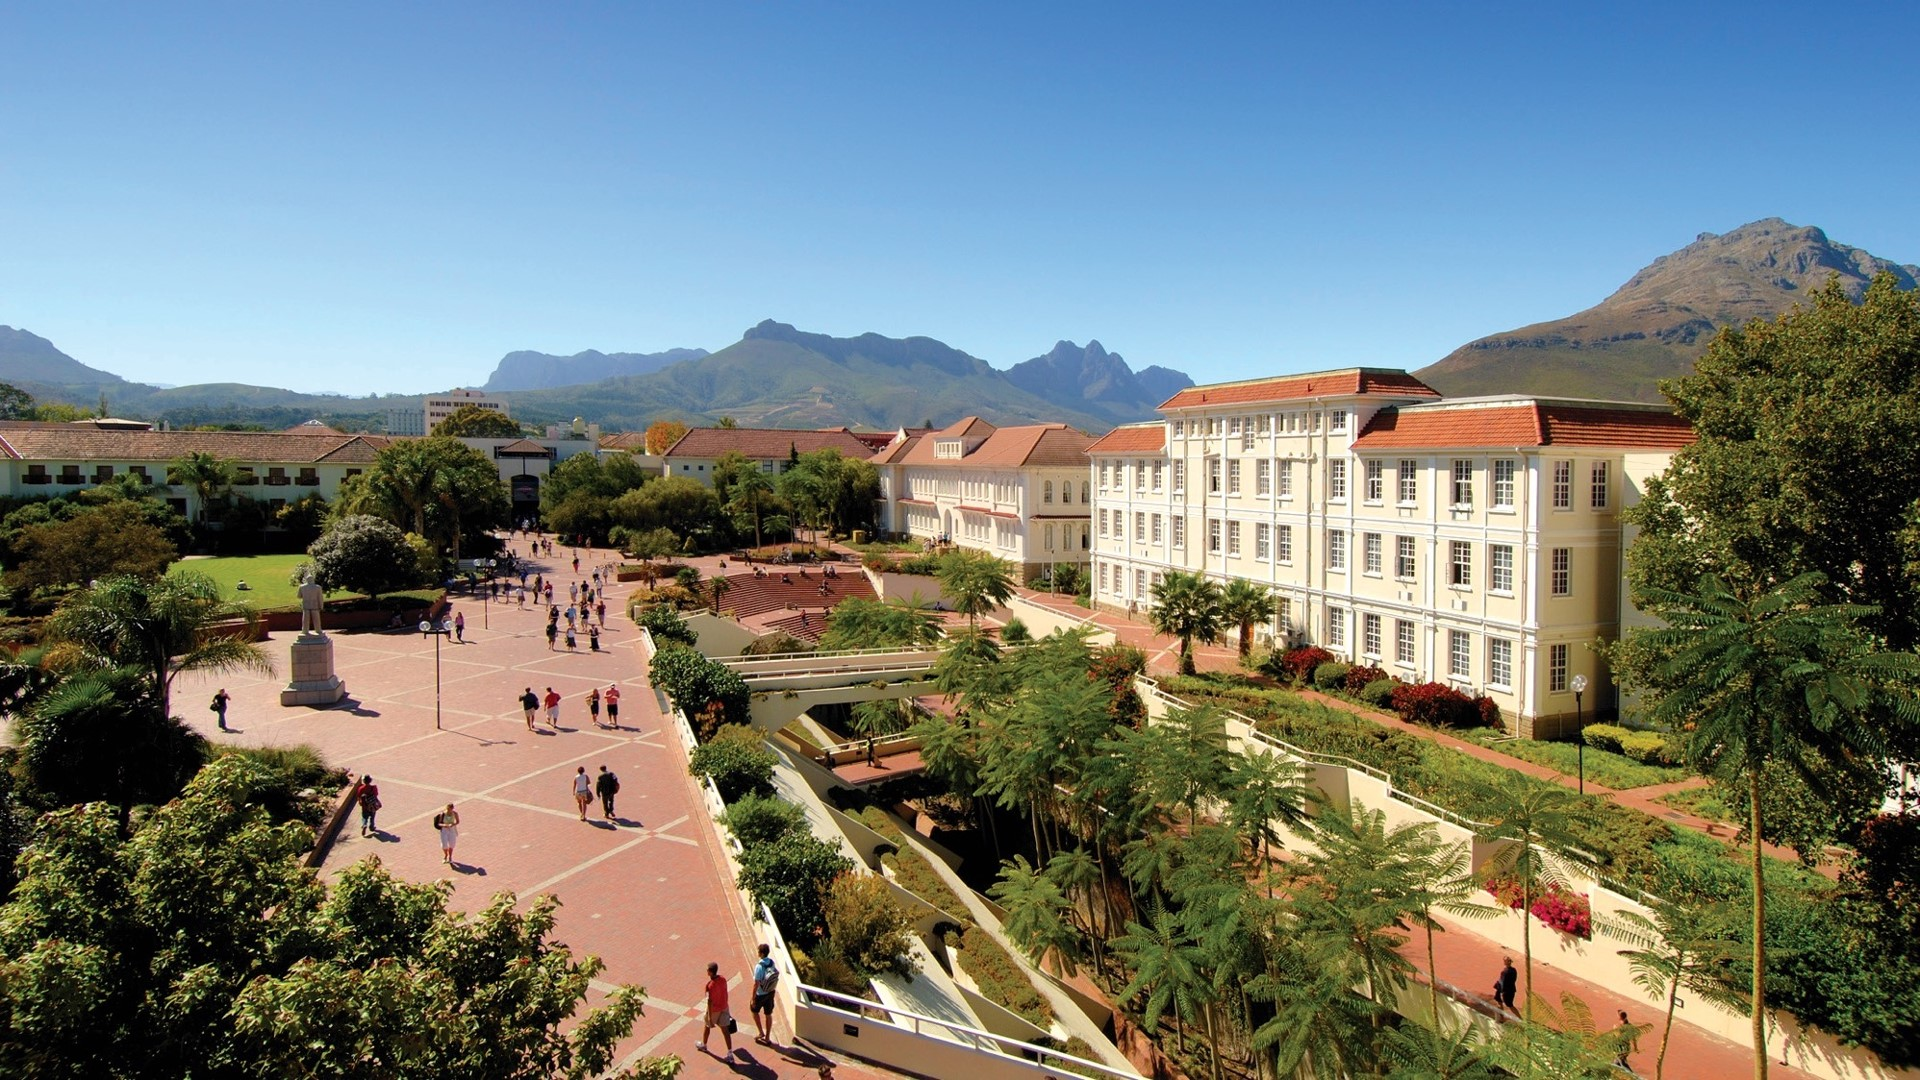
\includegraphics[width=1.2\hsize]{stb-campus-1}};
    \node[align=center,stbWine,font={\Huge\bfseries}] at (image.north) {Thank you\\};
\end{tikzpicture}
\end{frame}


\end{document}
